\section{Clustering Annotation}

Clustering task usually consists of tens or hundreds of targeted tokens that need to be clustered together. 

\subsection{View}

The entire window is separated into two parts. The left part (about 40\%) is used to display the document(s). We highlight all the targeted tokens with a grey background and white texts to make them more obvious and easier to notice. The right partition (about 60\%) is the operation area where user group related tokens together. Supporting manipulation methods will be introduced in Section \ref{sec:manipulation}. Each token has a corresponding node in the operation area. To bridge the connection between the text display and graphic chart, we label each token and its corresponding node with an index.

\subsection{Manipulation}
\label{sec:manipulation}
Our main manipulation method for clustering two nodes together is dragging nodes and merging into one group. It is the most intuitive operation for one without any instructions to merge two nodes. We will explain the select and drag, link add and remove, and color scheme in the following paragraphs.

\paragraph{\textsc{Select and Drag}\\}
Since we have two separate parts, one for displaying the text, the other for cluster and group manipulation, a proper selection must be supported in order to reduce user's eye movement between two parts. We adopt three mechanism to address this issue. First, if user click on one token, the corresponding node will be highlighted in red color. Similarly when user starts to drag a node, the token is also highlighted in red background. Second, to accelerate tracing from node to the actual text, once user start to drag a node, the display section will scroll to a proper position to let user easily read the context of this token. Third, as shown in Figure \ref{fig:abbrtext}, when drag event starts, an abbreviation text will be displayed under each node so that user can have a brief concept of what each node represents.

\begin{figure}
\begin{center}
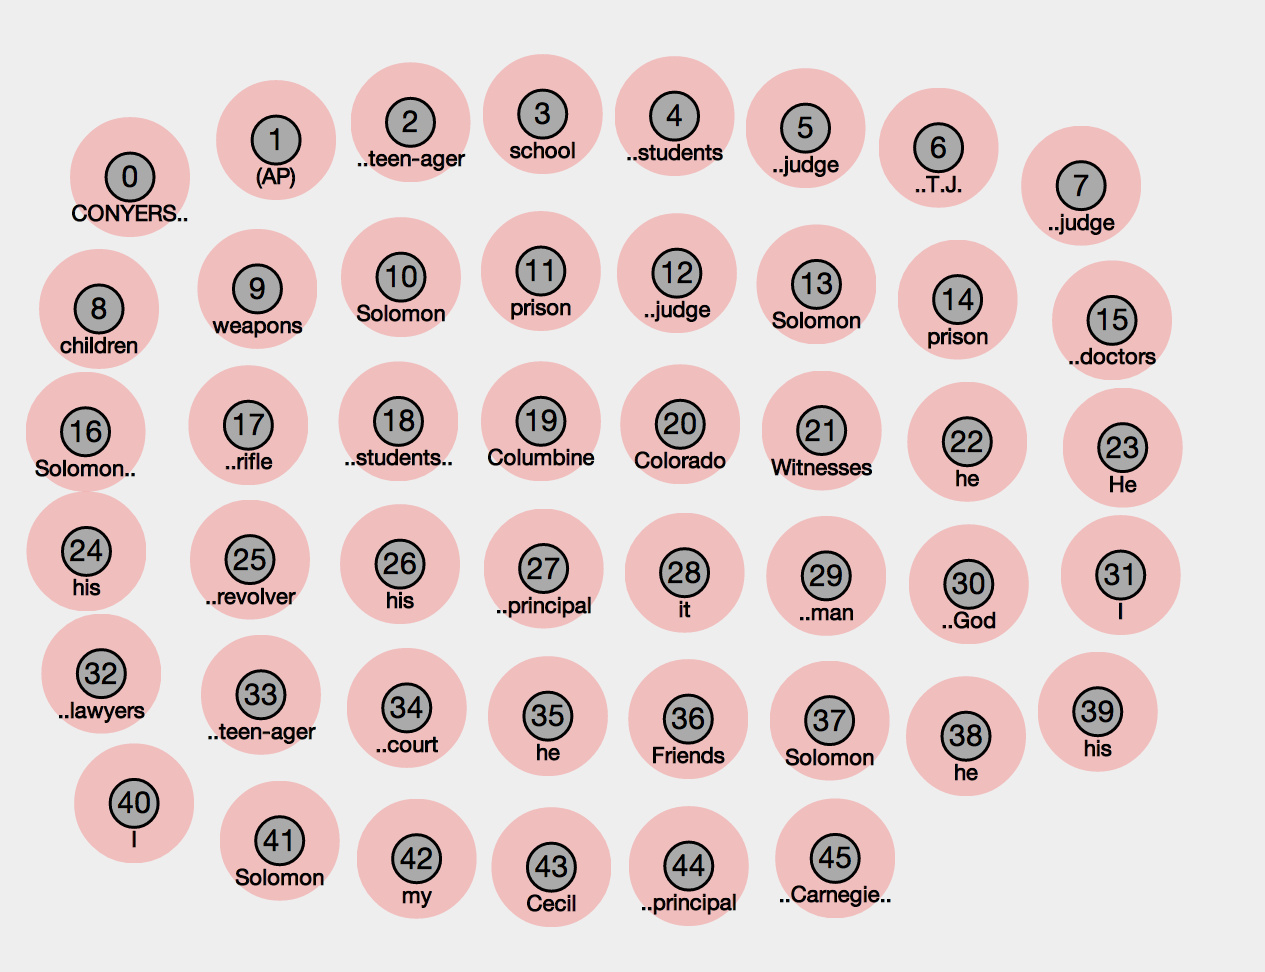
\includegraphics[height=4cm]{figs/abbrText.jpg}
\caption{Abbreviation text is displayed under each node after dragging starts.}
\label{fig:abbrtext}
\end{center}
\end{figure}

\paragraph{\textsc{Link Add and Remove}\\}

\paragraph{\textsc{Group Position}\\}

\paragraph{\textsc{Color Scheme}\\}